% Formato para un capítulo cualquiera

%Título del capítulo
\chapter{Introducción} 


Durante todo el siglo XX, en España, han ocurrido más de 7.000.000 de accidentes de tráfico \cite{sigloXX}, de los que en aproximadamente en 250.000 han habido víctimas mortales \cite{vidas}. No sabemos cuántos de ellos fueron por exceso de velocidad; sin embargo, fue, y es, la principal causa de éstos junto con el factor humano \cite{dgt-velocidad}. 

Durante ese tiempo se comenzaron a pensar soluciones para poder reducirlos, como la modificación de los límites de velocidad en la consecución de distintos gobiernos \cite{limites-velocidad}. Y fruto de ello, gracias a la evolución de la tecnología, surgieron los sistemas \ac{ISA} para regular la velocidad dentro del vehículo y ayudar así al conductor.

No todos los sistemas \ac{ISA} son iguales y su uso no es el mismo para cada vehículo. Hay algunos cuya función consiste en el reconocimiento y recomendación de la limitación de velocidad, y otros que actúan como un limitador de la velocidad inteligente \cite{2022}; depende de la marca y el modelo donde de implementen.

Actualmente se llevan utilizando durante bastante tiempo, y en 2022 serán obligatorios para los vehículos nuevos homologados en la Unión Europea. Modelos como el Mercedes Clase-S, el Peugeot 3008 y el Fiat 500X fueron pioneros usando esta tecnología \cite{2022}.

%Un siglo después, gracias a la evolución de la tecnología, se crean los sistemas \ac{ISA}, que permiten establecer una velocidad aproximada para ayudar al conductor en cualquier situación de la vía.

%TODO_DONE: No me convence el párafo, pasas de los accidentes a los ISA dando un gran salto. Los sistemsa ISA no han aparecido un siglo después, por cierto, llevan tiempo. Modifica el párrafo para hilar ambas cosas. ¿Cuántos accidentes se deben a excesos de velocidad? ¿Hay cifras? Regular la velocidad es importante, existen lo sistemas ISA. Habla de soluciones comerciales (hay muchos modelos de coches que los llevan, basados en sistemas de detección de señales de tráfico, GPS y meta información, sensores de proximidad, etc).


Con la creación de estos sistemas se estima que el número de accidentes se reduciría considerablemente, y más importante aún, el número de víctimas \cite{reduccion}.


Sin embargo, estos sistemas, a pesar de tener buenas prestaciones, presentan algunos problemas. Esto es debido a que la mayoría de sistemas \ac{ISA} están basados en combinar la posición \ac{GPS} con meta-información asociada a la misma, en relación a la velocidad máxima permitida en la vía. Es decir, el módulo ISA comienza localizando mediante GPS la posición del vehículo, para luego consultar para esa posición, qué velocidad es la máxima permitida en dicha vía. Los principales problemas que pueden surgir, siguiendo este procedimiento, son los siguientes:

\begin{itemize}
\item La información de la velocidad máxima de la vía puede que no esté actualizada, o que incluso sea incorrecta.
\item La precisión de la localización de los sistemas GPS en ocasiones puede resultar insuficiente para este tipo de sistemas. Por ejemplo, cuando circulamos por una vía de servicio paralela a una autovía, el sistema GPS puede no tener resolución suficiente para posicionarnos en el tipo de vía correcto. Nótese que los límites de velocidad son muy diferentes para estos dos tipos de vías (p. ej. 90 km/h versus 120 km/h), y el sistema ISA puede fallar.
\item No tienen en cuenta la situación real del tráfico, salvo si utilizan sensores de proximidad de otros vehículos, combinados con la información del GPS.
\end{itemize}


Es por ello que aquí presentamos un sistema basado en el procesado de imágenes, capaz de resolver (en gran medida) estos problemas: \[ISA^{2}\]
%TODO_DONE: ¿Cómo? Anticipa en qué se basa: procesado de imagen.


\section{¿Qué es $ISA^{2}$? ¿Cómo funciona?}


La principal novedad de $ISA^{2}$ frente a los otros sistemas \ac{ISA} reside en la capacidad para analizar la situación real y actual del tráfico, y predecir, en consecuencia, la velocidad apropiada para ese instante. No se parte de información asociada a coordinadas GPS, sino que se emplean técnicas de inteligencia artificial y visión por computador para reconocer la situación de tráfico real, y poder recomendar una velocidad al conductor. A continuación se pueden ver una serie de figuras con el proceso debidamente explicado:

\begin{figure}[H]
  \centering
  \begin{subfigure}[b]{0.4\linewidth}
    \includegraphics[width=\linewidth]{Figuras/Imagen_Original.eps}
    \caption{Imagen Original}
    \label{fig:ImgOrig}
  \end{subfigure}
    \begin{subfigure}[b]{0.45\linewidth}
    \includegraphics[width=\linewidth]{Figuras/Ejemplo_Imagen_Segmentada.eps}
    \caption{Imagen Segmentada}
    \label{fig:ImgSegm}
  \end{subfigure}
    \begin{subfigure}[b]{0.4\linewidth}
    \includegraphics[width=\linewidth]{Figuras/Ejemplo_Histograma.eps}
    \caption{Ejemplo del vector de características representado como un histograma}
    \label{fig:Hist}
  \end{subfigure}
      \begin{subfigure}[b]{0.4\linewidth}
    \includegraphics[width=\linewidth]{Figuras/SVR_Urban(Nivel_1).eps}
    \caption{Ejemplo de regresión final}
    \label{fig:Regre}
  \end{subfigure}
  \caption{Proceso de $ISA^{2}$}
\end{figure}

Para empezar usamos una cámara en la parte frontal del vehículo que va tomando imágenes con una cierta frecuencia (figura \ref{fig:ImgOrig}). Gracias a un sistema de \ac{SS}, conseguimos saber qué es cada cosa en cada foto, es decir; qué píxeles son los correspondientes a un vehículo, peatón, semáforo, acera, etc (figura \ref{fig:ImgSegm}). Con esa información se construye un vector de características (figura \ref{fig:Hist}) que será empleado por los módulos de inteligencia artificial para realizar una regresión o estimación de la velocidad a la que se debe circular(figura \ref{fig:Regre}).

%TODO_DONE: mejor que una imagen con solo datos de segmentación semántica, debes incluir una imagen donde se vea todo, desde la imagen original, a la segmentación semántica, y al proceso de extracción de características y la regresión final. Es para dar una idea gráfica del problema. Una vez la tengas, la metes y la comentas en el propio texto. Te dejo lo de abajo comentado para que lo cambies.

%He aquí un ejemplo de una imagen real \ref{fig:ImgOrig} y de la misma imagen procesada por el sistema de \ac{SS} \ref{fig:ImgSegm}:

%\begin{figure}[h]
%  \centering
%  \includegraphics[width=12cm]{Figuras/Imagen_Original.eps}
%  \caption{Imagen Original}
%  \label{fig:ImgOrig}
%\end{figure}

%\begin{figure}[h]
%  \centering
%  \includegraphics[width=12cm]{Figuras/Ejemplo_Imagen_Segmentada.eps}
%  \caption{Imagen Segmentada}
%    \label{fig:ImgSegm}
%\end{figure}


\section{Objetivo principal}


El objetivo principal de este proyecto es la optimización del sistema $ISA^{2}$, con respecto a la versión anterior. Para ello, partiremos de los recursos que tenemos de éste y buscaremos la mejor manera de hacerlo más práctico y eficiente. La principal mejora queremos acometerla en un incremento de la velocidad del sistema, pero sin perder de vista la precisión del mismo.
%TODO_DONE: Sergio, lo que tenías no eran objetivos. Debes poner aquí de forma muy clara los objetivos del trabajo fin de grado.



\section{Campos de aplicación}


Este proyecto será aplicable a los sistemas de transporte inteligentes, para ayudar a mejorar la seguridad vial, facilitando una solución para controlar la velocidad a la que deben circular los vehículos. A modo de resumen, podríamos destacar las siguientes aplicaciones:
\begin{enumerate}	
	\item Implementación de soluciones de adaptación de velocidad inteligente que avisen al conductor en función de la situación real del tráfico.
	\item Implementación de sistema de detección de situaciones peligrosas en función de la velocidad.
	\item Desarrollo de nuevas ayudas a la conducción más inteligentes.
\end{enumerate}

%\section{Medios disponibles}

%Dispondremos de las siguientes herramientas:

%\begin{enumerate}
%	\item Estación de trabajo con \textbf{GPU (NVIDIA 1080 TI)} para la realización de experimentos con sistema operativo \textbf{Ubuntu}.
%	\item Acceso a la librería de \textbf{Deep Learning} llamada \textbf{PyTorch} \cite{pytorch}
%	\item Acceso a la base de datos $ISA^2$ utilizada en la primera versión \cite{isa2} a través del siguiente enlace: \url{http://agamenon.tsc.uah.es/Personales/rlopez/data/isa2/index.html}.
%\end{enumerate}

%TODO: Falta por completar la introducción con un párrafo de cierre donde explicas cómo está organizada la memoria -> "Este documento está organizado de la siguiente forma. En el capítulo 2 blablabla. El capítulo 3 incluye blablabla..."
